%%%%%%%%%%%%%%%%%%%%%%%%%%%%%%%%%%%%%%%%%%%%%%%%%%%%%%%%%%%%%%%%%%%%%%%%%%%%%%%
%234567890123456789012345678901234567890123456789012345678901234567890123456789
%        1         2         3         4         5         6         7         

\documentclass[letterpaper, 10 pt, conference]{ieeeconf}  % Comment this line out if you need a4paper

%\documentclass[a4paper, 10pt, conference]{ieeeconf}      % Use this line for a4 paper

\IEEEoverridecommandlockouts
% This command is only needed if 
% you want to use the \thanks command

\overrideIEEEmargins

% Needed to meet printer requirements.

% See the \addtolength command later in the file to balance the column lengths
% on the last page of the document

% The following packages can be found on http:\\www.ctan.org
%\usepackage{graphics} % for pdf, bitmapped graphics files
%\usepackage{epsfig} % for postscript graphics files
%\usepackage{mathptmx} % assumes new font selection scheme installed
%\usepackage{times} % assumes new font selection scheme installed
%\usepackage{amsmath} % assumes amsmath package installed
%\usepackage{amssymb}  % assumes amsmath package installed

\usepackage[hidelinks]{hyperref}
\usepackage{graphicx}
\usepackage{subcaption}
\usepackage{ dsfont }
\usepackage{ amsmath }

\hyphenpenalty=100000

\title{\LARGE \bf
Dynamic Validation of Multi-robot Motion Planning Using a Distributed Receding Horizon Approach
}


\author{Jos\'{e} M. Mendes Filho$\,^{a,}\,^{b,}\,^{*}$, Eric Lucet$\,^{a}$ and David Filliat$\,^{b}$\\% <-this % stops a space
\thanks{$^{a}$ CEA, LIST, Interactive Robotics Laboratory, Gif-sur-Yvette, F-91191, France}
\thanks{$^{b}$ Unit\'{e} d'Informatique et d'Ing\'{e}nierie des Syst\`{e}mes, ENSTA Paristech, 828 bd des Marechaux, 91762, France}
\thanks{$^{*}$ corresponding author: {\tt\small jose.mendesfilho@cea.fr}}
}
% \thanks{*This work was not supported by any organization}% <-this % stops a space
% \thanks{$^{1}$Jos\'{e} M. Mendes Filho is with the CEA, LIST, Interactive Robotics Laboratory, Gif-sur-Yvette, F-91191, France
%         {\tt\small jose.mendesfilho@cea.fr}}%
% \thanks{$^{2}$Eric Lucet is with the CEA, LIST, Interactive Robotics Laboratory, Gif-sur-Yvette, F-91191, France
%         {\tt\small eric.lucet@cea.fr}}%
% \thanks{$^{3}$David Filliat is with the Unit\'{e} d'Informatique et d'Ing\'{e}nierie des Syst\`{e}mes, ENSTA Paristech, 828 bd des Marechaux, 91762, France
%                 {\tt\small david.filliat@ensta-paristech.fr}}%
%}


\begin{document}



\maketitle
\thispagestyle{empty}
\pagestyle{empty}


%%%%%%%%%%%%%%%%%%%%%%%%%%%%%%%%%%%%%%%%%%%%%%%%%%%%%%%%%%%%%%%%%%%%%%%%%%%%%%%%
\begin{abstract}

% This paper proposes the real-time implementation of an algorithm for collision-free motion planning based on a receding horizon approach, for the navigation of a team of mobile robots in the presence of obstacles of different shapes. The method is simulated with three robots. The impact of the parameters is studied with regard to computation time, obstacle avoidance and travel time.
This paper analyzes the real-time implementation of an algorithm for collision-free motion planning of a team of wheeled mobile robots in the presence of obstacles in a realistic enviromnent. Planning and navigation are simulated with three robots. Deviations from the planned motion caused by the system dynamics can be overcome by doing few changes in the optimization problem uderlying the planning algorithm and using a feedback controller.
\end{abstract}


%%%%%%%%%%%%%%%%%%%%%%%%%%%%%%%%%%%%%%%%%%%%%%%%%%%%%%%%%%%%%%%%%%%%%%%%%%%%%%%%
\section{INTRODUCTION}

% Context

The capability of defining a collistion-free motion plan for passing from one configuration to another is a crutial aspect of robotics that can be specially hard to solve for mobile multi-robot systems. A trending application that require this capability is the use of robotic systems in industrial supply chains for processing orders and optimizing the storage and distribution of products. For example, Amazon employs the Kiva mobile-robot system, and IDEA Groupe employs the Scallog system for autonomously processing client orders~\cite{Gizmag,supplychain}. Such logistics tasks became increasingly complex as sources of uncertainty, such as human presence, are admitted in the work environment.

%Problem

For efficiently solving the motion planning problem, different constraints must be taken into account, in particular, geometric, kinematic and dynamic constraints. The first constraints result from the need of preventing the robot to assume specific configurations in order to avoid collisions, communication loss, etc. Kinematic constraints derive directly from the mobile robot architecture implying, in particular, in nonholonomic constraints. Dynamics constraints come mainly from inertial effects and interaction between different bodies in contact.

In~\cite{MendesFilho2015}, a Distributed Receding Horizon Motion Planning is presented. It is intended for planning the motion of a team of nonholonomic mobile robots, in a partially known environment occupied by static obstacles, being efficient with respect to the travel time (amount of time to go from initial to goal configuration). However, only kinematic validation of that approach was done and its applicability in a more realistic scenario remained to be tested.

This work builds directly on that approach and aims to analyze that motion planning method in a realistic scenario. By means of a physics engine that can simulate rigid body dynamics (including collision detection), the aproach is tested, evaluated and improved. The improvements are meant to take effects such as inertia and sliding motion into account and overcome possible deviations between the executed and planned motion.

Related work (...)
% TODO

%The focus of this paper is to analyze the Receding Horizon Motion Planning presented in~\cite{MendesFilho2015} in a realistic scenario. By means of a physics engine that can simulate rigid body dynamics (including collision detection) the motion planning aproach can be tested, evaluated and improved. The improvements are meant to take effects such as inertia and sliding motion into account and overcome deviations between the executed and planned motion.

%A new implementation of the planning method was done using XDE (eXtended Dynamics Engine)~\cite{Merlhiot12}. Changes in the planner were needed so effects such as inertia and sliding motion that were neglected before could be taken into account.


%State of Art

% A great amount of work towards collision-free motion 
% planning for cooperative multi-robot systems has been proposed. That work can
% be split into centralized and distributed approaches.
% Centralized approaches are usually formulated as an optimal
% control problem that takes all robots in the team into account at once.
% This produces solutions closer to the optimal one than distributed approaches. However, the computation time, security vulnerability and communication 
% requirements can make it impracticable, specially for a great number of 
% robots~\cite{Borrelli2006}.

% Distributed methods based in probabilistic~\cite{Sanchez2002} and artificial 
% potential fields~\cite{Khatib1986} approaches, for instance, are computationally fast.
% However, they deal with collision avoidance as a cost function to be minimized.
% But rather than having a cost that increases as paths leading
% to collision are considered, collision avoidance should to be considered as hard constraints of the problem.


% Other distributed algorithms are based on receding horizon approaches.
% In \cite{Defoort2009} a brief comparison of the main distributed receding 
% methods is made as well as the presentation of the base approach extended in
% our work.
% In this approach each robot optimizes only its own 
% trajectory at each computation/update horizon. In order to
% avoid robot-to-robot collisions and lost of communication, neighbor robots 
% exchange information about their intended trajectories before 
% performing the update. Intended trajectories are computed by each robot
% ignoring constraints that take the other robots into account.

% Identified drawbacks of this approach are the dependence on 
% several parameters for achieving real-time performance and good solution 
% optimality, the difficulty to adapt it for handling dynamic obstacles, the 
% impossibility of bringing the robots to a precise goal state and the limited
% geometric representation of obstacles.

This paper outline is as follows. The second section gives an overview of the Distributed Receding Horizon Motion Planning. It shows how this approach manages to find motion plans that respect geometric and kinematics cosntraints while minimizing the travel time of each robot in the team. The third section proposes a simple change on the optimization problem uderlying the motion planning for providing better plans with respect to the system dynamics. It also proposes a feedback control that asymptotically stabilizes the tracking error. The forth section is dedicated to the dynamic simulation aspects and the results of using the proposed motion planning in that realistic scenario.   (...)
% TODO
Finally, in last section we present our conclusions and perspectives.

%The third section explains how the a simple change on the optimization problem uderlying the motion planning plus the addition of a feedback controller can provide a  realistic simulation. First a direct modification on the optimization problem uderlying the motion planning to take accelerations limits into account thus providing better plans with respect to the system dynamics.

\section{DITRIBUTED RECIDING HORIZON MOTION PLANNING}

As a team of robots evolves in their work enviroment they progressively perceive new obstacles in their way to their goal configuration. Thus, try to plan for the whole motion from initial to goal configurations is not a satisfying approach. Planning locally and replanning is more suitable for taking new information into account as it comes.

In the Distributed Reciding Horizon approach for motion planning, each robot in the team computes its own local plan. Two fundamental concepts of this approach are the planning horizon $T_p$ and update/computation horizon $T_c$. $T_p$ is the timespan for which a solution will be computed and $T_c$ is the time horizon during which a plan is executed while the next plan, valid for the next timespan $T_p$, is being computed. The problem of producing a motion plan for a $T_p$ horizon during the $T_c$ time interval is called
here a receding horizon planning problem.

For each receding horizon planning problem, the following steps are performed:
\paragraph*{Step 1}\label{step1} Each robot in the team computes it own intended solution trajectory (denoted $(\hat{q}_b(t), \hat{u}_b(t))$ with $q_b$ the configuration vector a robot $b$ and $u_b$ its input vector) by solving a constrained optimization problem that takes geometric and kinematics constraints into account. Coupling constraints, that is, constraints that involve solving a conflict between two robots such as collision or loss of communication, are ignored in this step.
\paragraph*{Step 2}\label{step2} Robots involved in a potential conflict (risk of collision, lost of communication) update their trajectories computed during \nameref{step1} by solving a second constrained optimization problem that additionally takes into account constraints for avoiding the conflict. This is done by using the intended trajectories of other robots computed in the previous step as an estimate of those robots' final trajectories. If a robot is not involved in any conflict, \nameref{step2} is not executed and its final solution trajectory is identical to the one estimated in \nameref{step1}.

All robots in the team use the same $T_p$ and $T_c$ for assuring that their intended trajectories begin at the same time and are valide for the same time horizon. However, this is not necessary condition.

For each of these steps and for each robot in the team, one constrained optimization problem is resolved. The cost function to be minimized in those optimization problems is the geodesic distance of a robot's current configuration to its goal configuration. This assures that the robots are driven towards their goal.

This two step scheme is explained in details in~\cite{Defoort2009} where constrained optimization problems associated to the receding horizon 
optimization problem are formulated.

However, when a robot arrives closer to its goal the receding horizon planning scheme does not produce the desired effect. For instance, near the goal, a plan for reaching it can possibly take less time than the $T_p$ planning horizon. 

In~\cite{MendesFilho2015} a termination procedure for reaching the goal is proposed. It takes the goal configuration as a hard constraint in the optimization problem and uses the time for reaching the goal as the cost function to be minimized.

Figure~\ref{fig:recedinghor} illustrates how plans would be generated through time by the receding horizon scheme with termination plan.

%\begin{figure}[thpb]
%	\centering
%	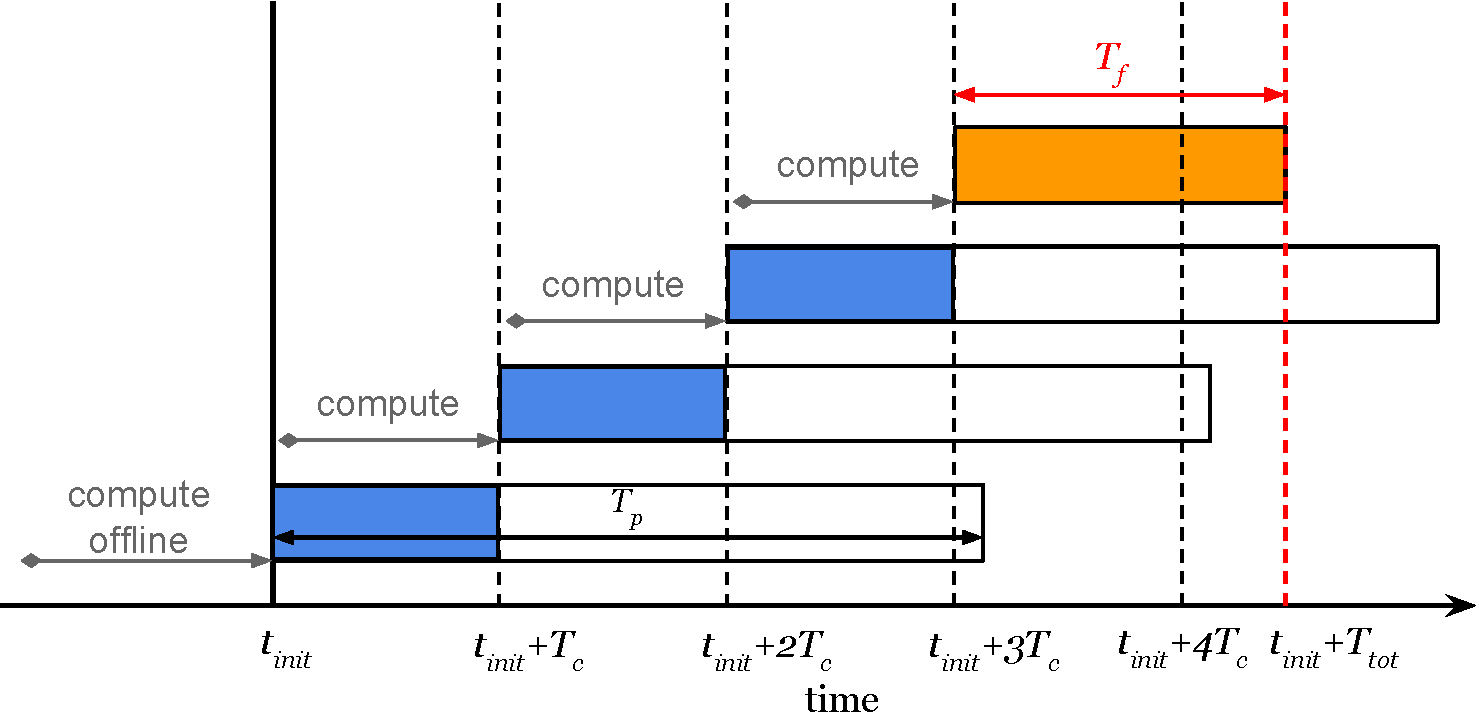
\includegraphics[width=\linewidth]{./images/MotionPlanning.pdf}
%	\caption{Receding horizon scheme with termination plan. The timespan $T_f$ represents the duration of the plan for reaching the goal configuration.}
%	\label{fig:recedinghor}
%\end{figure}

Although, the plans generated with this approach are not necessarily appropriated for 

% For evaluting whether or not \nameref{step2} must be performed, each robot must be able to compute a conflict list. This list identifies, for example, robots with whom the robot creating the list may collide in the next planning step. In order to do that the robots must know each other positions.


\mbox{}



%%%%%%%%%%%%%%%%%%%%%%%%%%%%%%%%%%%%%%%%%%%%%%%%%%%%%%%%%%%%%%%%%%%%%%%%%%%%%%%
\section{Predictive control law synthesis}

\subsection{Extended Model}

For finding a predictive control law an extended model which integrates the dynamics of the unicycle is needed. The model bellow in equation \ref{eq:extendedModel} can be used for that purpose:

\begin{eqnarray}
\underbrace{\left[\begin{array}{c}
\dot{x}\\
\dot{y}\\
\dot{\theta}\\
\dot{v}\\
\dot{\omega}
\end{array}\right]}_{\dot{q}} =
\underbrace{\left[\begin{array}{c}
v\cos\theta\\
v\sin\theta\\
\omega\\
\frac{p_3}{p_1}\omega^2 - \frac{p_4}{p_1}v\\
-\frac{p_5}{p_2}v\omega - \frac{p_6}{p_2}\omega
\end{array}\right]}_{f(q)}+
\underbrace{\left[\begin{array}{cc}
0 & 0\\
0 & 0\\
0 & 0\\
\frac{1}{p_1} & 0\\
0 & \frac{1}{p_2}
\end{array}\right]}_{g(q) = [g_1(q)\ g_2(q)]}
\underbrace{\left[\begin{array}{c}
u_1\\
u_2
\end{array}\right]}_{u}
\label{eq:extendedModel}
\end{eqnarray}

$q \in Q \subset \mathds{R}^n$ is the state vector and $u \in U \subset \mathds{R}^p$ the input.

%For later introducing the design of the predictive controller we may write the above system in the following form:
%\[
%\dot{q} = f(q) + \sum_{j=1}^pg_j(q)u_j
%\]
%which gives:
%
%\begin{eqnarray}
%\left[\begin{array}{c}
%\dot{x}\\
%\dot{y}\\
%\dot{\theta}\\
%\dot{v}\\
%\dot{\omega}
%\end{array}\right] = \left[\begin{array}{c}
%v\cos\theta\\
%v\sin\theta\\
%\omega\\
%\frac{p_3}{p_1}\omega^2 - \frac{p_4}{p_1}v\\
%-\frac{p_5}{p_2}v\omega - \frac{p_6}{p_2}\omega
%\end{array}\right]+
%\left[\begin{array}{c}
%0\\
%0\\
%0\\
%\frac{1}{p_1}\\
%0
%\end{array}\right]u_1+
%\left[\begin{array}{c}
%0\\
%0\\
%0\\
%0\\
%\frac{1}{p_2}
%\end{array}\right]u_2
%\label{eq:extendedModel}
%\end{eqnarray}

%with
%
%\begin{align*}
%q = \left[\begin{array}{c}
%x\\
%y\\
%\theta\\
%v\\
%\omega
%\end{array}
%\right]
%\end{align*}

The parameters vector $p \in \mathds{R}^6$ can be determined by system identification or based on properties of the unicycle such as mass, moment of inertia with respect to different axes, impedance of motors etc.

%To synthesize a control law that minimizes the quadratic error in position and orientation (in pose) over a time horizon $T$.

\subsection{Optimal predictive control}

The objective is to synthesize a control law that minimizes the quadratic error in position and orientation (i.e. pose) over a time horizon $T$ ahead of the current instant $t$.

Since only error in pose is to be minimized, the system output can be written as follows:

\[
h = \left[\begin{array}{c}
x\\
y\\
\theta
\end{array}
\right]
\]

And the error as:

\[
	e(t) =  h(t) - h_{\text{ref}}(t)
\]

where $h_{\text{ref}}(t)$ is derived from the trajectory planner output.

The criterion to be minimized represented by $J$ can be written as:

\begin{align*}
J = \sum_{i=1}^m J_i 
\end{align*}

with

\begin{align*}
J_i = \int_0^{T} (\hat{e}_i(t+\tau))^2d\tau
\end{align*}

where $\hat{e}_i(t+\tau)$ represents the prediction error at $t+\tau$ with $0 < \tau \leq T$.

To find the control law that minimizes $J$ is to find $u$ satisfying the equation:

\begin{align*}
\frac{\partial J}{\partial u} = 0_{p\times 1}
\end{align*}

For solving the above equation a expression for the prediction error must be defined and the criterion rewritten in a matrix form.

%Predictive control equation minimizing the position and orientation errors.

\subsection{Predictive error definition}

Using Taylor series, each of the coefficients of $h(t+\tau)$ can be written as bellow:

\begin{align*}
h_i(t+\tau) = \sum_{k=0}^{\rho_i} 
h^{(k)}_i(t)\frac{\tau}{k!} + R(\tau^{\rho_i})
\end{align*}

Rewriting in a matrix form and excluding the remainder term an approximation for the output $h_i$ is given bellow:

\begin{eqnarray}
h_i(t+\tau) \simeq \underbrace{\left[\begin{array}{ccccc}
1 & \tau & \frac{\tau^2}{2} & \dots & \frac{\tau^{\rho_i}}{{\rho_i}!}
\end{array}\right]}_{\Lambda_i}
\left[\begin{array}{c}
h_i(t)\\
\dot{h}_i(t)\\
\ddot{h}_i(t)\\
\vdots\\
h^{(\rho_i)}_i(t)
\end{array}\right]
\end{eqnarray}

Replacing the first matrix by the more compact notation $\Lambda_i$ and using the standard geometric notation for Lie derivatives the previous can be written as:

\begin{eqnarray}
h_i(t+\tau) \simeq \Lambda_i L_{h_i}
\end{eqnarray}

where

\begin{eqnarray*}
L_{h_i} = \left[\begin{array}{c}
L_f^{(0)}h_i(t)\\
L_f^{(1)}h_i(t)\\
\vdots\\
L^{({\rho_i}-1)}_fh_i(t)\\
L^{({\rho_i})}_fh_i(t)+L_gL_{h_i}^{({\rho_i}-1)}h_i(t)u(t)
\end{array}\right]
\end{eqnarray*}

%and, inductively:

\begin{eqnarray*}
\left\lbrace\begin{array}{lcl}
L_f^{(k)} h_i & = & L_fL_f^{(k-1)}h_i = \frac{\partial L_f^{\rho-1}h_i}{\partial q}(q)f(q)\\
L_f^{(0)}h_i & = & h_i\\
\end{array}\right.
\end{eqnarray*}

%\begin{align}
%u = \argmin_u\sum_{i=1}^{m}J_i
%\end{align}

The second term in the prediction error expression, $h_{\text{ref}}(t+\tau)$, can be analogously written as:

\begin{eqnarray}
h_{\text{ref},i}(t+\tau) \simeq \Lambda_i
\underbrace{\left[\begin{array}{c}
h_{\text{ref},i}(t)\\
\dot{h}_{\text{ref},i}(t)\\
\ddot{h}_{\text{ref},i}(t)\\
\vdots\\
h^{({\rho_i})}_{\text{ref},i}(t)
\end{array}\right]}_{L_{h_{\text{ref},\,i}}}
\end{eqnarray}

$L_{h_{\text{ref},\, i}}$ is supposed to be known from the trajectory planner output for any $\rho_i$.

\subsection{Control law equation}

After some (a lot of) algebraic manipulation we can show that:

\[
\frac{\partial J}{\partial u} = 0 \Rightarrow u = -(D^TD)^{-1}D^TKE
\]

with $D$ the decoupling matrix, $K$ the the gain matrix and $E$ the prediction error matrix defined as bellow:

\begin{eqnarray}
D = 
\left[\begin{array}{ccc}
L_{g_1}L_f^{\rho_1-1}h_1 & \dots & L_{g_p}L_f^{\rho_1-1}h_1\\
\vdots & \ddots & \vdots\\
L_{g_1}L_f^{\rho_m-1}h_m & \dots & L_{g_p}L_f^{\rho_m-1}h_m
\end{array}\right]
\end{eqnarray}

\begin{eqnarray}
E = 
\left[\begin{array}{c}
h_1 - h_{\text{ref},\,1}\\
\vdots\\
L_f^{(\rho_1)}h_1 - h^{(\rho_1)}_{\text{ref},\,1}\\
\vdots\\
h_m - h_{\text{ref},\,m}\\
\vdots\\
L_f^{(\rho_m)}h_m - h^{(\rho_m)}_{\text{ref},\,m}
\end{array}\right]
\end{eqnarray}

\begin{eqnarray}
K = 
\left[
\begin{array}{ccc}
\Pi^{ss}_1 & & 0\\
& \ddots &\\
0 & & \Pi^{ss}_m
\end{array}\right]^{-1}
\left[\begin{array}{ccc}
\Pi^{s}_1 & & 0\\
& \ddots &\\
0 & & \Pi^{s}_m
\end{array}\right]
\end{eqnarray}

with $\Pi^{s}_i$ the last line of the matrix $\Pi_i$ and $\Pi^{ss}_i$ the last element of the vector $\Pi^{s}_i$. 

$\Pi_i$ being defined as:

%& \frac{\tau^{(\rho_i-1)+1}}{((\rho_i-1)+1)(\rho_i-1)!}

\begin{align}
&\Pi_i = \int^{T_i}_0\Lambda_i^T\Lambda_id\tau\\
&=  \left[\begin{array}{cccccc}
T_i & \frac{T_i^2}{2} & \dots & \frac{T_i^{(\rho_i-1)+1}}{((\rho_i-1)+1)(\rho_i-1)!} & \frac{T_i^{\rho_i+1}}{(\rho_i+1)\rho_i!}\\
\frac{T_i^2}{2} & \frac{T_i^3}{3} & \dots &  \frac{T_i^{((\rho_i-1)+1)+1}}{(((\rho_i-1)+1)+1)(\rho_i-1)!} & \frac{T_i^{(\rho_i+1)+1}}{((\rho_i+1)+1)\rho_i!}\\
& & \ddots & & \\
\frac{T_i^{\rho_i+1}}{(\rho_i+1)\rho_i!} & & \dots & \frac{T_i^{(\rho_i+(\rho_i-1))+1}}{((\rho_i+(\rho_i-1))+1)\rho_i!(\rho_i-1)!} & \frac{T_i^{(\rho_i+\rho_i)+1}}{((\rho_i+\rho_i)+1)\rho_i!\rho_i!}
\end{array}\right]
\end{align}

The MIMO (Multiple Input Multiple Output) system has relative degree vector $\rho = [\rho_1(t) \dots \rho_m(t)]$ for all $q$ in the neighborhood of $q^0$ if:

\begin{itemize}
\item $L_{gj}L_f^kh_i(x) = 0$ for all $1 \leq j \leq p$, for all $k < \rho_i-1$, for all $1 \leq i \leq m$ and for all $q$ in the neighborhood of $q^0$
\item the product $D^TD$ is non-singular, $D$ being the decoupling matrix of dimension $m \times p$, given by:

\begin{eqnarray}
D = 
\left[\begin{array}{ccc}
L_{g_1}L_f^{\rho_1-1}h_1 & \dots & L_{g_p}L_f^{\rho_1-1}h_1\\
\vdots & \ddots & \vdots\\
L_{g_1}L_f^{\rho_m-1}h_m & \dots & L_{g_p}L_f^{\rho_m-1}h_m
\end{array}\right]
\end{eqnarray}
\end{itemize}

A way of trying to find a vector $\rho$ for our particular system is by computing $L_{g_i}L_f^kh_j$ for $k$ beginning at $0$ and incrementing it until the conditions above are satisfied.

For $\rho = [1\ 1\ 1]$, $L_{g_i}L_f^0h_j = L_{g_i}h_j = 0$ for all $1 \leq i \leq p$, for all $1 \leq j \leq m$.

%\begin{eqnarray}
%\left\lbrace\begin{array}{lcl}
%L_{g_1}h_1 & = & [1\ 0\ 0\ 0\ 0\ 0][0\ 0\ 0\ 1/p_1\ 0]^T = 0\\
%L_{g_1}h_2 & = & [0\ 1\ 0\ 0\ 0\ 0][0\ 0\ 0\ 1/p_1\ 0]^T = 0\\
%L_{g_1}h_3 & = & [0\ 0\ 1\ 0\ 0\ 0][0\ 0\ 0\ 1/p_1\ 0]^T = 0
%\end{array}\right.
%\end{eqnarray}
%
%\begin{eqnarray}
%\left\lbrace\begin{array}{lcl}
%L_{g_2}h_1 & = & [1\ 0\ 0\ 0\ 0\ 0][0\ 0\ 0\ 0\ 1/p_2]^T = 0\\
%L_{g_2}h_2 & = & [0\ 1\ 0\ 0\ 0\ 0][0\ 0\ 0\ 0\ 1/p_2]^T = 0\\
%L_{g_2}h_3 & = & [0\ 0\ 1\ 0\ 0\ 0][0\ 0\ 0\ 0\ 1/p_2]^T = 0
%\end{array}\right.
%\end{eqnarray}

For computing $L_{g_i}L_f^kh_j$ with $\rho = [2\ 2\ 2]$ we need first $L_fh_j$:

\begin{eqnarray}
\left\lbrace\begin{array}{lcl}
L_{f}h_1 & = & [1\ 0\ 0\ 0\ 0\ 0]f(q) = v\cos\theta\\
L_{f}h_2 & = & [0\ 1\ 0\ 0\ 0\ 0]f(q) = v\sin\theta\\
L_{f}h_3 & = & [0\ 0\ 1\ 0\ 0\ 0]f(q) = \omega
\end{array}\right.
\end{eqnarray}

Computing now $L_{g_j}L_fh_j$ we obtain:

\begin{eqnarray}
\left\lbrace\begin{array}{lcl}
L_{g_1}L_{f}h_1 & = & [0\ 0\ -v\sin\theta\ \cos\theta\ 0\ 0]g_1(q) = \cos\theta/p_1\\
L_{g_1}L_{f}h_2 & = & [0\ 0\ v\cos\theta\ \sin\theta\ 0\ 0]g_1(q) = \sin\theta/p_1\\
L_{g_1}L_{f}h_3 & = & [0\ 0\ 0\ 0\ 0\ 1]g_1(q) = 0
\end{array}\right.
\end{eqnarray}

\begin{eqnarray}
\left\lbrace\begin{array}{lcl}
L_{g_2}L_{f}h_1 & = & [0\ 0\ -v\sin\theta\ \cos\theta\ 0\ 0]g_2(q) = 0\\
L_{g_2}L_{f}h_2 & = & [0\ 0\ v\cos\theta\ \sin\theta\ 0\ 0]g_2(q) = 0\\
L_{g_2}L_{f}h_3 & = & [0\ 0\ 0\ 0\ 0\ 1]g_2(q) = 1/p_2
\end{array}\right.
\end{eqnarray}

Which gives the following decoupling matrix:

\begin{eqnarray}
D = 
\left[\begin{array}{cc}
\frac{\cos\theta}{p_1} & 0\\
\frac{\sin\theta}{p_1} & 0\\
0 & \frac{1}{p_2}
\end{array}\right]
\end{eqnarray}

and consequently:

\begin{eqnarray}
D^TD = 
\left[\begin{array}{cc}
\frac{1}{p_1^2} & 0\\
0 & \frac{1}{p_2^2}
\end{array}\right]
\end{eqnarray}

which is non-singular for all $p_1, p_2 \neq 0$.

\begin{eqnarray}
K =
\left[\begin{array}{ccccccccc}
\frac{10}{3T_1^2} & \frac{5}{2T_1} & 1 & 0 & 0 & 0 & 0 & 0 & 0\\
0 & 0 & 0 & \frac{10}{3T_2^2} & \frac{5}{2T_2} & 1 & 0 & 0 & 0\\
0 & 0 & 0 & 0 & 0 & 0 & \frac{10}{3T_3^2} & \frac{5}{2T_3} & 1
\end{array}\right]
\end{eqnarray}

\begin{eqnarray}
E =
\left[\begin{array}{c}
x - x_{\text{ref}}\\
v\cos\theta - v_{\text{ref}}\cos\theta_{\text{ref}}\\
\left(\frac{p_3}{p_1}\omega^2 - \frac{p_4}{p_1}v\right)\cos\theta - v\omega\sin\theta - a_{\text{ref}}\cos{\theta_{\text{ref}}}\\
y - y_{\text{ref}}\\
v\sin\theta - v_{\text{ref}}\sin{\theta_{\text{ref}}}\\
\left(\frac{p_3}{p_1}\omega^2 - \frac{p_4}{p_1}v\right)\sin\theta + v\omega\cos\theta - a_{\text{ref}}\sin{\theta_{\text{ref}}}\\
\theta - \theta_{\text{ref}}\\
\omega - \omega_{\text{ref}}\\
-\frac{p_5}{p_2}v\omega - \frac{p_6}{p_2}\omega - \alpha_{\text{ref}}\\
\end{array}\right]
\end{eqnarray}

\[
u(q, q_{\text{ref}}, a_{\text{ref}}, \alpha_{\text{ref}}, T, p) = -(D^TD)^{-1}D^TKE
\]

\begin{equation}
\dot{q}(t) = f(q(t), u(t)) \Rightarrow\\
\left\lbrace\begin{array}{lcl}
\dot{x} = u_1\cos\theta\\
\dot{y} = u_1\sin\theta\\
\dot{\theta} = u_2\cos\theta
\end{array}\right.
\end{equation}

For the feedback control, a specific method applicable to unicycle-type robots for tracking a reference vehicle with the same kinematics was used~\cite{siciliano2008springer}. The configuration trajectory $t \longmapsto q_b^*(t)$ can be considered as the solution to the robot's kinematic model for the specific control input trajectory $t \longmapsto u_b^*(t)$. Therefore, those trajectories can be used as references ((\ref{eq:refconfig}) and (\ref{eq:refctrl})) in the control law in (\ref{eq:ctrllaw}) that renders the system globally asymptotically stable under certain conditions\footnote{The orientation error between the physical robot and the reference robot is smaller than $\pi$/2, $u_{1,r}$ is a bounded differentiable function whose derivative is bounded and which does not tend to zero as t tends to infinity}.

\begin{equation}\label{eq:refconfig}
q_b^*(t) = [x_r\ y_r\ \theta_r]^T
\end{equation}

\begin{equation}\label{eq:refctrl}
u_b^*(t) = [u_{1,r}\ u_{2,r}]^T
\end{equation}

\begin{equation}\label{eq:ctrllaw}
\left\lbrace\begin{array}{lcl}
u_1 = (-k_1|u_{1,r}|(w_1 + w_2w_3) + u_{1,r})\cos^{-1}(\theta-\theta_r)\\
u_2 = (-k_2u_{1,r}w_2 - k_3|u_{1,r}|w_3)\cos^2(\theta-\theta_r) + u_{2,r}
\end{array}\right.
\end{equation}
with $w_1 = x - x_r$, $w_2 = y - y_r$, $w_3 = \tan(\theta - \theta_r)$.

The gains $k_1$, $k_2$ and $k_3$ were tunned using pole placement based on the linearization of the system and control.
32
For simplicity, the observation of the configurations of each robot was considered exact. This is not an issue if we consider that the robot can detect landmarks in its enviromnent whose absolute positions are known in advance and that data fusion and filtering fsrom different sensors can bound the observation error to small values.




\begin{table}[h]
\caption{An Example of a Table}
\label{table_example}
\begin{center}
\begin{tabular}{|c||c|}
\hline
One & Two\\
\hline
Three & Four\\
\hline
\end{tabular}
\end{center}
\end{table}


   \begin{figure}[thpb]
      \centering
      \framebox{\parbox{3in}{We suggest that you use a text box to insert a graphic (which is ideally a 300 dpi TIFF or EPS file, with all fonts embedded) because, in an document, this method is somewhat more stable than directly inserting a picture.
      }}
      %\includegraphics[scale=1.0]{figurefile}
      \caption{Inductance of oscillation winding on amorphous
       magnetic core versus DC bias magnetic field}
      \label{figurelabel}
   \end{figure}
   

\section{CONCLUSIONS}


\addtolength{\textheight}{-12cm} 
% This command serves to balance the column lengths
% on the last page of the document manually. It shortens
% the textheight of the last page by a suitable amount.
% This command does not take effect until the next page
% so it should come on the page before the last. Make
% sure that you do not shorten the textheight too much.

%%%%%%%%%%%%%%%%%%%%%%%%%%%%%%%%%%%%%%%%%%%%%%%%%%%%%%%%%%%%%%%%%%%%%%%%%%%%%%%



%%%%%%%%%%%%%%%%%%%%%%%%%%%%%%%%%%%%%%%%%%%%%%%%%%%%%%%%%%%%%%%%%%%%%%%%%%%%%%%



%%%%%%%%%%%%%%%%%%%%%%%%%%%%%%%%%%%%%%%%%%%%%%%%%%%%%%%%%%%%%%%%%%%%%%%%%%%%%%%
%\section*{APPENDIX}


%\section*{ACKNOWLEDGMENT}

%%%%%%%%%%%%%%%%%%%%%%%%%%%%%%%%%%%%%%%%%%%%%%%%%%%%%%%%%%%%%%%%%%%%%%%%%%%%%%%

\bibliographystyle{IEEEtran}
\bibliography{ref}

\end{document}
